\documentclass{standalone}
\usepackage{tikz}
\usepackage{pgfplots}
\pgfplotsset{width=32cm,height=18cm,compat=1.3}
\pgfplotsset{every tick label/.append style={font=\Huge}}
\usepackage{filecontents}

\usetikzlibrary{patterns}

\definecolor{citrine}{rgb}{0.89, 0.82, 0.04}

\begin{document}
	\centering
		\vspace{1.5em}
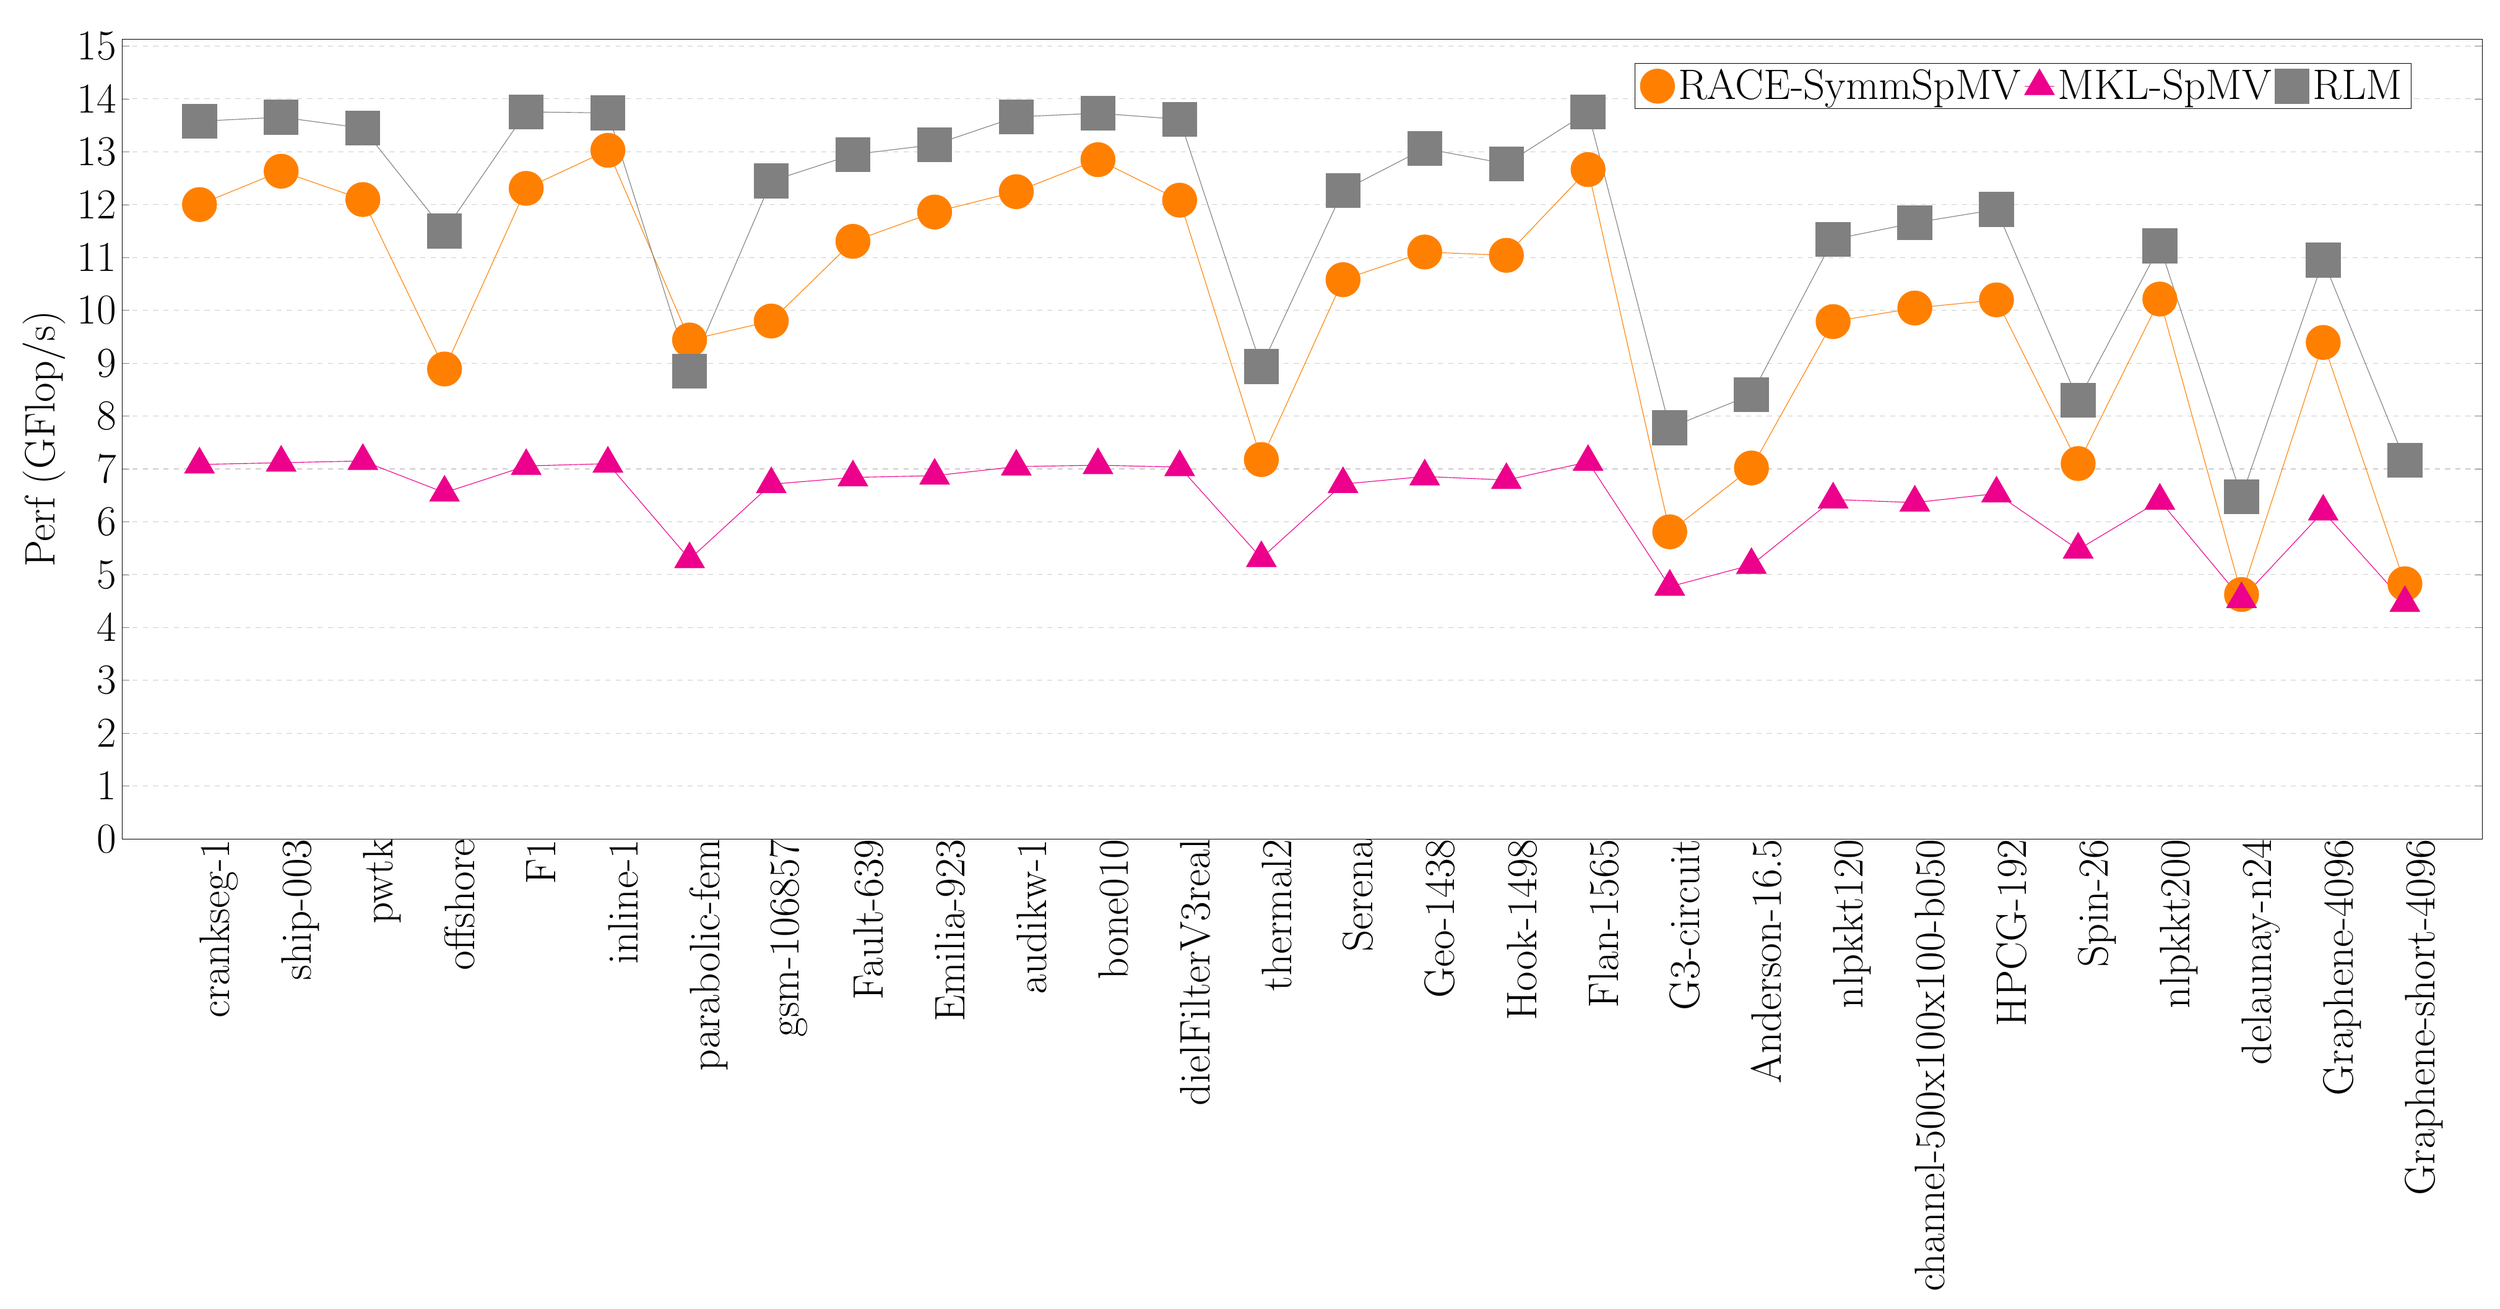
\begin{tikzpicture}
		%	\node at (13.25,15) {\LARGE{}};
			\begin{axis}[
		%	xmin=0.25, xmax=7.25,
			ymin=0, %ymax=3.25,
			xtick={1, 2, 3, 4, 5, 6, 7, 8, 9, 10, 11, 12, 13, 14, 15, 16, 17, 18, 19, 20, 21, 22, 23, 24, 25, 26, 27, 28},
		%	ytick={0,0.5,1,1.5,2,2.5,3},
			xticklabels={crankseg-1, ship-003, pwtk, offshore, F1, inline-1, parabolic-fem, gsm-106857, Fault-639, Emilia-923, audikw-1, bone010, dielFilterV3real, thermal2, Serena, Geo-1438, Hook-1498, Flan-1565, G3-circuit, Anderson-16.5, nlpkkt120, channel-500x100x100-b050, HPCG-192, Spin-26, nlpkkt200, delaunay-n24, Graphene-4096, Graphene-short-4096},
			width  = 50cm,
			height = 18cm,
			major x tick style = transparent,
			%	minor ytick={1, 5, 10, 15, 20, 25, 30 ,35,40},
			grid = minor,	
			%add_bar_commands
			ymajorgrids = true,
			grid style={dashed, gray!40},
			ylabel = {\Huge{Perf (GFlop/s)}},
		%	symbolic x coords={Graphene-2048-2048, Graphene-4096-4096, Spin-24-24-24},
			x tick label style={rotate=90, anchor=north east, inner sep=0mm, font={\Huge}},
			tick label style={font={\Huge}},
			scaled y ticks = false,
			enlarge x limits=0.035,
			legend cell align=left,
			legend style={font=\Huge},
			legend columns=-1,
			legend style={
				%at={(1,1.05)},
				%anchor=south east,
				%column sep=1ex,
				legend pos=north east
			},
			%spl_legend_code
			title= {\Huge\scalebox{1.5}{{}}}
			]

\addplot[mark=*, mark size=10pt, mark options={orange}, draw=orange ] plot coordinates{(1,12.001241) (2,12.632607) (3,12.096590) (4,8.890258) (5,12.308086) (6,13.027954) (7,9.439195) (8,9.797964) (9,11.305451) (10,11.860212) (11,12.245165) (12,12.850634) (13,12.084667) (14,7.176575) (15,10.580104) (16,11.103660) (17,11.040916) (18,12.663604) (19,5.809891) (20,7.017762) (21,9.787395) (22,10.044041) (23,10.198226) (24,7.101122) (25,10.213585) (26,4.623104) (27,9.392370) (28,4.827286)};
\addplot[mark=triangle*, mark size=10pt, mark options={magenta}, draw=magenta ] plot coordinates{(1,7.083106) (2,7.117153) (3,7.150255) (4,6.551354) (5,7.054848) (6,7.099324) (7,5.291437) (8,6.709915) (9,6.838865) (10,6.871915) (11,7.043145) (12,7.070277) (13,7.033526) (14,5.311964) (15,6.712824) (16,6.856778) (17,6.789662) (18,7.131561) (19,4.770986) (20,5.182545) (21,6.421885) (22,6.362534) (23,6.534070) (24,5.473422) (25,6.398243) (26,4.537544) (27,6.191554) (28,4.464146)};
\addplot[mark=square*, mark size=10pt, mark options={gray}, draw=gray ] plot coordinates{(1,13.578052263635199) (2,13.65493316565024) (3,13.44628627227418) (4,11.50270180170624) (5,13.754909468814018) (6,13.73488805180514) (7,8.849498616835636) (8,12.446182807945874) (9,12.948473557567187) (10,13.135270512521675) (11,13.660186160839144) (12,13.729827668414957) (13,13.61438110888941) (14,8.936517101213635) (15,12.266428629748441) (16,13.06267700040604) (17,12.771974331145039) (18,13.755685901937294) (19,7.779433252562224) (20,8.402259494089943) (21,11.340446668397544) (22,11.656606158032847) (23,11.908526291666126) (24,8.296004307427339) (25,11.220436445916942) (26,6.474584637640949) (27,10.949022059480217) (28,7.1608522058141455)};
	%addplot cmd

	\legend{RACE-SymmSpMV, MKL-SpMV, RLM}

	\end{axis}			
\end{tikzpicture}

\end{document}

